\begin{figure}[htbp]
\centering
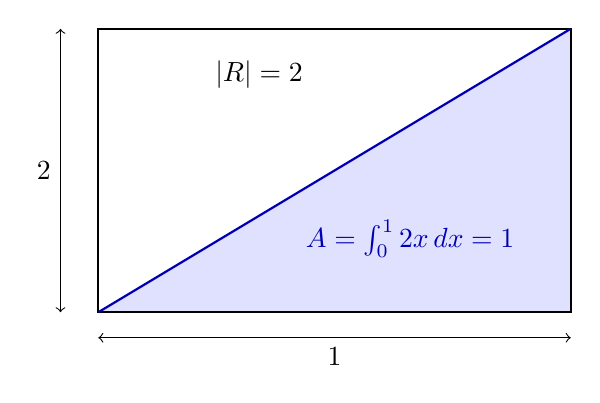
\begin{tikzpicture}[x=6cm,y=1.8cm]
  \fill[blue!12] (0,0) -- plot[domain=0:1,samples=60] (\x,{2*\x}) -- (1,0) -- cycle;
  \draw[thick] (0,0) rectangle (1,2);
  \draw[thick,blue!70!black,domain=0:1,samples=60] plot (\x,{2*\x});
  \draw[<->] (0,-0.18) -- (1,-0.18) node[midway,below] {$1$};
  \draw[<->] (-0.08,0) -- (-0.08,2) node[midway,left] {$2$};
  \node[blue!70!black] at (0.66,0.52) {$A=\int_0^1 2x\,dx=1$};
  \node at (0.34,1.68) {$|R|=2$};
\end{tikzpicture}
\caption{El cociente entre el área sombreada y el área del rectángulo es la probabilidad de aceptación.}\label{fig:area}
\end{figure}